\documentclass[english,onecolumn]{IEEEtran}
\usepackage[T1]{fontenc}
\usepackage[latin9]{luainputenc}
\usepackage[letterpaper]{geometry}
\geometry{verbose}
\usepackage{amsfonts}
\usepackage{babel}

\usepackage{extarrows}
\usepackage[colorlinks]{hyperref}
\usepackage{listings}
\usepackage{xcolor}
\usepackage[ruled,linesnumbered]{algorithm2e}

\usepackage{amsmath,graphicx}
\usepackage{subfigure} 
\usepackage{cite}
\usepackage{amsthm,amssymb,amsfonts}
\usepackage{textcomp}
\usepackage{bm}
\usepackage{booktabs}
\usepackage{listings}


\lstdefinestyle{mystyle}{
    numberstyle=\color{green},
    numbers=left,                    
    numbersep=5pt,                  
    showspaces=false,                
    showstringspaces=false,
    showtabs=false,                  
    tabsize=2
}

\lstset{style=mystyle}

\providecommand{\U}[1]{\protect\rule{.1in}{.1in}}
\topmargin            -18.0mm
\textheight           226.0mm
\oddsidemargin      -4.0mm
\textwidth            166.0mm
\def\baselinestretch{1.5}

\begin{document}

\begin{center}
	\textbf{{\Large SI231 - Matrix Computations, Fall 2020-21}}\\
	Homework Set \#2\\
   \texttt{Prof. Yue Qiu and Prof. Ziping Zhao} \\
	\texttt{\textbf{Name:}}   	\texttt{ aaa }  		\hspace{1bp}
	\texttt{\textbf{Major:}}  	\texttt{ Master in CS } 	\\
	\texttt{\textbf{Student No.:}} 	\texttt{ 2018123456}     \hspace{1bp}
	\texttt{\textbf{E-mail:}} 	\texttt{ aaa@shanghaitech.edu.cn}
\par\end{center}


\noindent
\rule{\linewidth}{0.4pt}
{\bf {\large Acknowledgements:}}
\begin{enumerate}
    \item Deadline: \textbf{2020-10-11 23:59:00}
    \item Submit your homework at \textbf{Gradescope}. Entry Code: \textbf{MY3XBJ}. Also, make sure that your gradescope account is your \textbf{school e-mail}.
    Homework \#2 contains two parts, the theoretical part the and the programming part.
    \item About the the theoretical part:
    \begin{enumerate}
            \item[(a)] Submit your homework in \textbf{Homework 2} in gradescope. Make sure that you have assigned the correct pages for the problems in the outline.
            \item[(b)] Your homework should be uploaded in the \textbf{PDF} format, and the naming format of the file is not specified.
            \item[(c)] No handwritten homework is accepted. You need to use \LaTeX. (If you have difficulty in using \LaTeX, you are allowed to use \textbf{Word} for the first and the second homework to accommodate yourself.)
            \item[(d)] Use the given template and give your solution in English. Solution in Chinese is not allowed. 
        \end{enumerate}
  \item About the programming part:
  \begin{enumerate}
      \item[(a)] Submit your codes in \textbf{Homework 2 Programming part} in gradescope.
      \item[(b)] Details of requirements in programming are listed in remarks of Problem 6, please read it carefully before you start to program.
  \end{enumerate}
  \item \textbf{No late submission is allowed.}
\end{enumerate}
\rule{\linewidth}{0.4pt}
\newpage 
\section{General Linear System}
\noindent\textbf{Problem 1}   \textcolor{blue}{(6 points + 9 points)}
\vspace*{3mm}

\noindent Let $\mathbf{A} = \begin{bmatrix}
	1 & 0 & 1 & 2\\
	-2 & 4 & -6 & 0\\
	3 & 1 & 14 & -1\\
	-1 & 7 & -5 & 3
	\end{bmatrix} \in\mathbb{R}^{4\times 4}\;$ and
	$\mathbf{B} = \begin{bmatrix}
	1 & 2 & 3 & -1\\
	2 & 3 & 1 & 1\\
	2 & 2 & 2 & -1\\
	5 & 5 & 2 & 3
	\end{bmatrix} \in\mathbb{R}^{4\times 4}\;.$
\begin{enumerate}
	\item 
	For {\bf A} and ${\bf b} = (-1,2,5,3)^T\in \mathbb{R}^4$, 
	find $\mathcal{N}({\bf A}),\, \mathcal{R}({\bf A})$, then solve ${\bf Ax} = {\bf b}$.
	\item 
	For {\bf B} and 
	${\bf b} = (1,1,1,2)^T \in \mathbb{R}^4$, solve the linear equation system ${\bf Bx} = {\bf b}$ 
	with Gauss Elimination, LU decomposition, and LU decomposition with partial pivoting, respectively. (Although not required, you are highly encouraged to write down your solution procedures in detail.)
\end{enumerate}

\noindent\textbf{Solution.}\\
\textbf{To TAs: I am so sorry that I have to write my ICC paper these days, so I don't have enough time to type my solutions in details. It will be appreciated if you can accept my undetailed solutions. Thank you very much.}
\begin{enumerate}
    \item First we find the row echelon form of A
    \begin{align*}
\begin{pmatrix}
1 & 0 & 1 & 2 \\ 
0 & 1 & -1 & 1 \\ 
0 & 0 & 1 & -\frac{2}{3} \\ 
0 & 0 & 0 & 0
\end{pmatrix} 
    \end{align*}
    Thus we have
    \begin{align*}
	\mathcal{N}(A)=r
	\begin{pmatrix}
	-\frac{8}{3} \\ -\frac{1}{3} \\ \frac{2}{3} \\1
	\end{pmatrix}, 
	\mathcal{R}(A)= s
	\begin{pmatrix}
	1 \\ -2 \\ 3 \\ -1
	\end{pmatrix}
	 + 	t\begin{pmatrix}
	 0 \\4 \\ 1 \\ 7
	 \end{pmatrix} + u	\begin{pmatrix}
	 1 \\ -6 \\ 14 \\ -5
	 \end{pmatrix}\quad r,s,t,u\in R
	\end{align*}
	Then we find the special solution $Ax^\star=b$ through augmented matrix
	$$\begin{pmatrix}
		1 & 0 & 1 & -1 \\ 
		-2 & 4 & -6 & 2 \\ 
		3 & 1 & 14 & 5 \\ 
		-1 & 7 & -5 & 3
	\end{pmatrix} \Rightarrow x^\star = (-\frac{5}{3},\frac{2}{3},\frac{2}{3},0)^T$$
	So we can express $x$ as follows:
	$$x=\begin{pmatrix}
	-\frac{5}{3} \\ \frac{2}{3} \\ \frac{2}{3} \\ 0
	\end{pmatrix} + r
	\begin{pmatrix}
	-\frac{8}{3} \\ -\frac{1}{3} \\ \frac{2}{3} \\1
	\end{pmatrix}, r\in R$$
    \item 
    \begin{itemize}
    	\item Gaussian Elimination:\\
    	First we write the augmented matrix
    	$$\begin{pmatrix}
    	1 & 2 & 3 & -1 & 1 \\ 
    	2 & 3 & 1 & 1 & 1 \\ 
    	2 & 2 & 2 & -1 & 1 \\ 
    	5 & 5 & 2 & 3 & 2
    	\end{pmatrix} $$
    	Then apply Gaussian elimination to get the ref of $B$
  		$$\begin{pmatrix}
  		1 & 2 & 3 & -1 & 1 \\ 
  		0 & 1 & 5 & -3 & 1 \\ 
  		0 & 0 & 1 & -\frac{5}{6} & \frac{1}{6} \\ 
  		0 & 0 & 0 & 1 & 0
  		\end{pmatrix} \Rightarrow x = (\frac{1}{6},\frac{1}{6},\frac{1}{6},0)^T$$
  		\item LU decomposition without pivoting\\
 		First we get the LU decompostion of B
 		$$L=\begin{pmatrix}
 		1 &  &  &  \\ 
 		2 & 1 &  &  \\ 
 		2 & 2 & 1 &  \\ 
 		5 & 5 & 2 & 1
 		\end{pmatrix},\quad U= \begin{pmatrix}
 		1 & 2 & 3 & -1 \\ 
 		& -1 & 5 & 3 \\ 
 		&  & 6 & -5 \\ 
 		&  &  & 3
 		\end{pmatrix} $$
 		Then we solve $Lz = b$
 		$$z = \begin{pmatrix}
 		1 \\ 
 		-1 \\ 
 		1 \\ 
 		0
 		\end{pmatrix} $$
 		Finally, we solve $Ux= z$
		 $$x = \begin{pmatrix}
		\frac{1}{6} \\ 
		\frac{1}{6} \\ 
		\frac{1}{6}\\ 
		0
		\end{pmatrix} $$	
		\item LU decompsition with pivoting
		 First we get U of  B by Guassian elimination
		$$\quad U= \begin{pmatrix}
		5 & 5 & 2 &3 \\ 
		& 1 & \frac{1}{5} & -\frac{1}{5} \\ 
		&  & \frac{12}{5} & -\frac{7}{5} \\ 
		&  &  & -\frac{3}{2}
		\end{pmatrix} $$
		Then we find L and P
		$$L=\begin{pmatrix}
			1 &  &  &  \\ 
			\frac{2}{5} & 1 &  &  \\ 
			\frac{1}{5} & 1 & 1 &  \\ 
			\frac{2}{5} & 0 & \frac{1}{2} & 1
		\end{pmatrix},P =\begin{pmatrix}
		0 & 0 & 0 & 1 \\ 
		0 & 1 & 0 & 0 \\ 
		1 & 0 & 0 & 0 \\ 
		0 & 0 & 1 & 0
		\end{pmatrix} $$
		Then we solve $Lz = Pb$
		$$z = \begin{pmatrix}
		2 \\ 
		\frac{1}{5} \\ 
		\frac{2}{5} \\ 
		0
		\end{pmatrix} $$
		Finally, we solve $Ux= z$
		$$x = \begin{pmatrix}
		\frac{1}{6} \\ 
		\frac{1}{6} \\ 
		\frac{1}{6}\\ 
		0
		\end{pmatrix} $$

    \end{itemize}
\end{enumerate}

\newpage
\section{Understanding Various Matrix Decompositions}
\noindent\textbf{Problem 2} \textcolor{blue}{(10 points)}

\noindent Consider the following symmetric matrix ${\bf A}\in \mathbb{R}^{4\times 4}$,
	\begin{align*}
		\mathbf{A}=
		\begin{bmatrix}
			a&a&a&a\\
			a&b&b&b\\
			a&b&c&c\\
			a&b&c&d
		\end{bmatrix}\,.
	\end{align*}
Give the LU decomposition of $\mathbf{A}$.
Then describe under which conditions $\bf{A}$ is nonsingular, according to the results of LU decomposition.

\noindent \textbf{Solution.}
First we find the LU decopmsition of matrix A
$$L=\begin{pmatrix}
1 &  &  &  \\ 
1 & 1 &  &  \\ 
1 & 1 & 1 &  \\ 
1 & 1 & 1 & 1
\end{pmatrix},\quad U = \begin{pmatrix}
a & a & a & a \\ 
& b-a & b-a & b-a \\ 
&  & c-b & c-b \\ 
&  &  & d-c
\end{pmatrix}  $$
A is nonsingular $\Leftrightarrow$ $det(A)\ne 0 \Leftrightarrow det(L)det(U)\ne 0$. Thus we have
$$a(b-a)(c-b)(d-c) \ne 0$$
This gives $a\ne b \ne c \ne d \ne 0$

\newpage
\noindent\textbf{Problem 3} \textcolor{blue}{(5 points + 10 points)}
\begin{enumerate}
	\item Consider a $3\times 3$ matrix
	\[
	\mathbf{A} = \begin{bmatrix}
		2& 2&4 \\
		1&5&1\\
		1&1&8
	\end{bmatrix}\,,
	\] find the LDM (also called LDU) decomposition of $\mathbf{A}$, i.e., factor $\mathbf{A}$ as $\mathbf{A}=\mathbf{L}\mathbf{D}\mathbf{M}^T$ (or $\mathbf{A}=\mathbf{L}\mathbf{D}\mathbf{U}$), where $\mathbf{L}\in\mathbb{R}^{3\times 3}$ is lower triangular with unit diagonal entries, $\mathbf{D}\in\mathbb{R}^{3\times 3}$  is  a diagonal matrix, and $\mathbf{M}\in\mathbb{R}^{3\times 3}$ is lower triangular with unit diagonal entries ($\mathbf{U}\in\mathbb{R}^{3\times 3}$ is upper triangular with unit diagonal entries).
	
	\item Consider a $3\times 3$ matrix
	\[
	\mathbf{B} = \begin{bmatrix}
		8& 1&1 \\
		1&5&1\\
		4&2&2
	\end{bmatrix}\,,
	\] find the UL decomposition  of $\mathbf{B}$, 
	i.e., factor $\mathbf{B}$ as $\mathbf{B} = \mathbf{UL}$,
	where $\mathbf{U}\in\mathbb{R}^{3\times 3}$ is upper triangular with unit diagonal entries and $\mathbf{L}\in\mathbb{R}^{3\times 3}$ is lower triangular.\\
	\textbf{Hint:}  $\mathbf{B}=\mathbf{P}\mathbf{A}\mathbf{P}$, where $\mathbf{P}$ is a unit anti-diagonal matrix \footnote{{\textbf{Anti-diagonal matrix:} An anti-diagonal matrix is a square matrix where all the entries are zero except those on the diagonal going from the lower left corner to the upper right corner, known as the anti-diagonal. For example, 
			\[
			\text{adiag}(a_1,\ldots,a_n) = \begin{bmatrix}
				0 & 0 & \cdots & 0 & a_1 \\
				0 & 0 & \cdots  & a_2 & 0 \\
				\vdots &  \vdots & \ddots & \vdots &\vdots \\
				a_n & 0 & \cdots &  \cdots& 0
			\end{bmatrix}\,,
			\]
			and consequently, unit anti-diagonal matrix means $\text{adiag}(1,\ldots,1)$, also known as the \textbf{exchange matrix} or the \textbf{permutation matrix}. 
	}}.
\end{enumerate}
\noindent\textbf{Solution.}
\begin{enumerate}
    \item First we find the LU decompistion of A
    $$L= \begin{pmatrix}
    1 &  &  \\ 
    \frac{1}{2} & 1 &  \\ 
    \frac{1}{2} & 0 & 1
    \end{pmatrix}, \quad U=\begin{pmatrix}
    2 & 2 & 4 \\ 
    & 4 & -1 \\ 
    &  & 6
    \end{pmatrix} $$
    Then we decompose $U$ into $DM$
    $$A=LDM^T=\begin{pmatrix}
1 &  &  \\ 
\frac{1}{2} & 1 &  \\ 
\frac{1}{2} & 0 & 1
\end{pmatrix}\begin{pmatrix}
2 &  &  \\ 
& 4 &  \\ 
&  & 6
\end{pmatrix} \begin{pmatrix}
1 & 1 & 2 \\ 
& 1 & -\frac{1}{4} \\ 
&  & 1
\end{pmatrix} $$
    \item Denote unit anti-diagonal matrix as $P$, we have
    \begin{align*}
    PAP &= PLDUP\\
    &= PLPD'PUP\\
    &=(PLPD)'(PUP)\\
    &\triangleq  U'L'
    \end{align*}
    So we find the $UL$ decomposition of $B$
    $$B=\begin{pmatrix}
    1 & 0 & \frac{1}{2} \\ 
    & 1 & \frac{1}{2} \\ 
    &  & 1
    \end{pmatrix}\begin{pmatrix}
    6 &  &  \\ 
    -1 & 4 &  \\ 
    4 & 2 & 2
    \end{pmatrix}  $$
\end{enumerate}

\newpage
\noindent\textbf{Problem 4} \textcolor{blue}{(7 points + 6 points + 7 points + 5 points)}

\noindent Given a matrix $\mathbf{A}\in\mathbb{R}^{n\times n}$, suppose that the LDM (LDU) decomposition of $\mathbf{A}$ exists, prove that
\begin{enumerate}
	\item the LDM (LDU) decomposition of $\mathbf{A}$ is \textit{uniquely} determined;
	\item if $\mathbf{A}$ is a symmetric matrix, then its LDM (LDU) decomposition must be $\mathbf{A}=\mathbf{L}\mathbf{D}\mathbf{L}^T$, which is called LDL (LDL$^T$) decomposition in this case;
	\item $\mathbf{A}$ is a symmetric and positive definite matrix if and only if its Cholesky decomposition exists (i.e., there exists a matrix $\mathbf{G}\in\mathbb{R}^{n\times n}$ such that $\mathbf{A}=\mathbf{G}\mathbf{G}^T$, where $\mathbf{G}$ is lower triangular with \textit{positive} diagonal entries);
	\item if $\mathbf{A}$ is a symmetric and positive definite matrix, then its Cholesky decomposition is \textit{uniquely} determined.	
\end{enumerate}

\textbf{Hints:}  
\begin{enumerate}
    \item The existence of the LDM (LDU) decomposition implies the non-singularity of the matrix.
    \item You can directly utilize the following lemmas,
\begin{itemize}
    \item the inverse (if it exists) of a lower (resp. upper) triangular matrix is also lower (resp. upper) triangular;
    \item the product of two lower (resp. upper) triangular matrices is lower (resp. upper) triangular;
    \item also, if such two lower (resp. upper) triangular matrices have unit diagonal entries, then their product also has unit diagonal entries.
\end{itemize}
\end{enumerate}

  

\noindent\textbf{Solution.}
\begin{enumerate}
    \item Assume that $A = L_1D_1U_1=L_2D_2U_2$. Then 
    $$D_2^{-1}L_2^{-1}L_1D_1=U_2U_1^{-1}$$
    RHS is the multiplication of upper triangular matrix thus also a upper triangular matrix, while LHS is a lower triangular matrix. This implies both side are diagonal matrix. Because $U_1,U_2$ have unit diagonal entries, RHS is also a upper triangular matrix with unit diagonal entries. This gives $$U_2U_1^{-1}=I, L_2^{-1}L_1=D_2D_1^{-1}, L_2^{-1}L_1=D_2D_1^{-1} = I$$
    Therefore, we have 
    $$U_2U_1^{-1}=L_2^{-1}L_1=D_2D_1^{-1}=I$$
    This implies $U_1=U_2,L_1=L_2,D_1=D_2$. Q.E.D.
    \item $A=LDM^T$ implies $M^{-1}AM^{-T} = M^{-1}LD$, which is both symmetric and triangular and therefore diagonal. Since $D$ is nonsingular, this implies $M^{-1}L$ is also diagonal. But $M^{-1}L$ is unit lower triangular. This implies $M^{-1}L=I$, which is equivalent to $A = LDL^T$. Q.E.D.
    \item '$\Rightarrow$'\\
    By the conclusion from 1) and 2), A has a unique $LDL^T$ decomposition. Since the principal minor of A is always $>0$ and $det(A)= det(L)^2det(D)$, we know that all diagnoal entry of the diagonal matrix $D$ are $>0$ (This is easy to proof by reduction, I omit here for time and space consideration). Given this, we let $G = LD^{\frac{1}{2}}$. Thus
    $$A = GG^T$$
  	'$\Leftarrow$'\\
  	$A = GG^T$ implies $A=GG^T = A^T$ is symmetric. Since $det(G) = \Pi_i d_i >0, Gx=0$ has non-trivial solution, that is $Gx\ne 0, G^Tx \ne 0$ when $x\ne 0$. Then
  	$$x^TAx = x^T(G^T)^TG^Tx = (G^Tx)\cdot(G^Tx) > 0\,\,(since\,\, G^Tx \ne 0),\forall x\ne 0$$
  	Therefore A is a symmetric and positive definite matrix. Q.E.D. 
    \item We assume that $A = G_1G_1^T = G_2G_2^T$. Then we have 
    $$G_2^{-1}G_1=G_1^{-T}G_2^T$$
    The LHS is lower triangular matrix and the RHS is an upper triangular matrix. So we have
    $$G_2^{-1}G_1=G_1^{-T}G_2^T=I$$
    This implies $G_1=G_2$, by which we have proved Cholesky decomposition is uniquely determined.
\end{enumerate}

\newpage
\noindent\textbf{Problem 5}
\textcolor{blue}{(10 points + 5 points)}

\noindent Consider matrix ${\bf A} \in \mathbb{R}^{n\times n}$ in the following form,
\[
\mathbf{A} = 
\begin{bmatrix}
	b_1 & c_1 &  0  &  0 & 0  & 0 \\
	a_2 & b_2 & c_2 &  0 & 0  & 0 \\
	0   & a_3 & b_3 & c_3 & 0 & 0 \\
	0   & 0 & \ddots & \ddots& \ddots&0\\
	\vdots & \vdots & \ddots& a_{n-1}& b_{n-1}& c_{n-1}\\
	0 & 0 & \cdots & 0 & a_{n} & b_n 
\end{bmatrix}\,,
\]
where $a_j$, $b_j$, and $c_j$ are non-zero entries.
The matrix in such form is known as a \textbf{Tridiagonal Matrix} in the sense that it contains three diagonals.
\begin{enumerate}
	\item LU decomposition is particularly efficient in the case of tridiagonal matrices. Find the LU decomposition of $\mathbf{A}$ (derivation is expected) and try to complete the Algorithm \ref{alg: lu_tri}.
\begin{algorithm}[htbp]
\SetKwInOut{Input}{Input}\SetKwInOut{Output}{Output}
\label{alg: lu_tri}
\caption{LU decomposition for tridiagonal matrices}
\SetAlgoLined
\Input{Tridiagonal matrix $\mathbf{A}\in \mathbb{R}^{n\times n}$.}
\Output{LU decomposition of $\mathbf{A}$.}
\text{$L=eye(n)$; $t=zeros(n,1)$; $U=A$;}\\
\text{\textbf{for} $k=1:1:n-1$}\\
\text{~~~ $rows = k+1:\min\{k+p,n\}$;}\\
\text{~~~ $cols = k+1:\min\{k+q,n\}$;}\\
\text{~~~ $t(rows) = U(rows:k)/U(k,k)$;}\\
\text{~~~ $U(rows,cols) = U(rows,cols)-t(rows)\star U(k,cols)$;}\\
\text{~~~ $U(rows,k)=0$;}\\
\text{~~~ $L(rows,k)=t(rows)$;}\\
\textbf{end;}
\end{algorithm}
\item
Consider symmetric tridiagonal matrices
\[
\mathbf{A} = \begin{bmatrix}
    1 & 1 & 0\\
    1 & 2 & 1 \\
    0 & 1 & 2 
\end{bmatrix}
\quad \text{and  }
\mathbf{B}= \begin{bmatrix}
    a & a & 0 \\
    a & a+b & b \\
    0 & b & b+c
\end{bmatrix}\,,
\]
and give the LU decompositions and the LDL$^T$ (also known as the LDL) decompositions of $\mathbf{A}$ and $\mathbf{B}$ respectively.
\end{enumerate}
\noindent\textbf{Solution.}
\begin{enumerate}
    \item 

    \item
    \begin{itemize}
    	\item [A]
    	$$U=\begin{pmatrix}
    	1 &  &  \\ 
    	0& 1 &  \\ 
    	0& -1 & 1
    	\end{pmatrix} 
    	\begin{pmatrix}
    	1 &  &  \\ 
    	-1& 1 &  \\ 
    	0& 0 & 1
    	\end{pmatrix}
    	\begin{pmatrix}
    	1 &1  &0  \\ 
    	1& 2 &1  \\ 
    	0& 1& 2
    	\end{pmatrix}=\begin{pmatrix}
    	1 &1  &0  \\ 
    	& 1 & 1 \\ 
    	&  & 1
    	\end{pmatrix}$$
    	$$L=\begin{pmatrix}
    	1 &  &  \\ 
    	1& 1 &  \\ 
    	0& 0 & 1
    	\end{pmatrix}
    	\begin{pmatrix}
    	1 &  &  \\ 
    	0& 1 &  \\ 
    	0& 1 & 1
    	\end{pmatrix}=\begin{pmatrix}
    	1 &  &  \\ 
    	1& 1 &  \\ 
    	0 & 1 & 1
    	\end{pmatrix}$$
    	
    	    	$$A=LU =\begin{pmatrix}
    	1 &  &  \\ 
    	1& 1 &  \\ 
    	0 & 1 & 1
    	\end{pmatrix}\begin{pmatrix}
    	1 &1  &0  \\ 
    	& 1 & 1 \\ 
    	&  & 1
    	\end{pmatrix}$$
    	
    	$$A=LDL^T =\begin{pmatrix}
    	1 &  &  \\ 
    	1& 1 &  \\ 
    	0 & 1 & 1
    	\end{pmatrix}\begin{pmatrix}
    	1 &  &  \\ 
    	& 1 &  \\ 
    	&  & 1
    	\end{pmatrix} \begin{pmatrix}
    	1 &1  &0  \\ 
    	& 1 & 1 \\ 
    	&  & 1
    	\end{pmatrix}$$
    	\item [B] 
    	$$U=\begin{pmatrix}
    	1 &  &  \\ 
    	0& 1 &  \\ 
    	0&  -\frac{a}{b}& 1\end{pmatrix}
    	\begin{pmatrix}
    	1 &  &  \\ 
    	-1& 1 &  \\ 
    	0&  0& 1\end{pmatrix}
    	\begin{pmatrix}
    	a &a  &  \\ 
    	a& a+b &b  \\ 
    	&  b& b+c\end{pmatrix}=    	\begin{pmatrix}
    	a & a & 0 \\ 
    	& b &  b\\ 
    	& & b+c-a\end{pmatrix}$$
    	$$L=    	\begin{pmatrix}
    	1 &  &  \\ 
    	1& 1 &  \\ 
    	0&  0& 1\end{pmatrix}    	\begin{pmatrix}
    	1 &  &  \\ 
    	0& 1 &  \\ 
    	0& \frac{a}{b}& 1\end{pmatrix}=    	\begin{pmatrix}
    	1 &  &  \\ 
    	1& 1 &  \\ 
    	0&  \frac{a}{b}& 1\end{pmatrix}$$
    	$$A = LU = \begin{pmatrix}
    	1 &  &  \\ 
    	1& 1 &  \\ 
    	0&  \frac{a}{b}& 1\end{pmatrix}\begin{pmatrix}
    	a & a & 0 \\ 
    	& b &  b\\ 
    	& & b+c-a\end{pmatrix}$$
    	$$A=LDL^T=\begin{pmatrix}
    	1 &  &  \\ 
    	1& 1 &  \\ 
    	0&  \frac{a}{b}& 1\end{pmatrix}\begin{pmatrix}
    	a &  &  \\ 
    	& b &  \\ 
    	& & b+c-a\end{pmatrix}\begin{pmatrix}
    	1 & 1 & 0 \\ 
    	& 1 & 1\\ 
    	& & 1\end{pmatrix}$$
    \end{itemize}    
\end{enumerate}

\newpage
\section{Programming}
\noindent\textbf{Problem 6}
\textcolor{blue}{(5 points + 15 points)}

\noindent In this problem, we explore  the efficiency of the LU method together with the classical linear system solvers we have learnt in linear algebra. 

\begin{enumerate}
	\item Derive the complexity of the LU decomposition. Particularly, how many flops does the LU decomposition require? The corresponding pseudo code (in {\sf Matlab}) is provided as follows: 
\begin{lstlisting}[language=Matlab]
function [L,U]= Naive_lu(A) 
    n = size(A,1)
    L = eye(n)
    U = A 
    for k=1:n-1
        for j=k+1:n
            L(j,k)=U(j,k)/U(k,k)
            U(j,k:n)=U(j,k:n)-L(j,k)*U(k,k:n)
        end
    end
    for k=2:n
        U(k,1:k-1)=0
    end
end
\end{lstlisting}
\item 
\textbf{Programming part:} 
Randomly generate a non-singular matrix $\mathbf{A}\in\mathbb{R}^{n\times n}$ and a vector $\mathbf{b}\in\mathbb{R}^{n\times 1}$, then program the following  methods to solve $\mathbf{Ax=b}$: 
\begin{itemize}
  \item {\bf The inverse method:} Use the inverse of $\mathbf{A}$ to solve the problem, which can be written as,
  \[
  \mathbf{x}=\mathbf{A}^{-1}\mathbf{b}\,.
  \]
  \item {\bf Cramer rule:} Suppose $\mathbf{x}=[x_1,\dots,x_n]^T$, and we denote $\mathbf{A}_{-i}(\mathbf{b})$ the matrix that we replace the $i$-th column of $\mathbf{A}$ with $\mathbf{b}$. Then we have
    \[
      x_i=\frac{\det(\mathbf{A}_{-i}(\mathbf{b}))}{\det(\mathbf{A})}, i=1,\dots,n\,.
    \]
  \item {\bf Gauss Elimination:} We perform row operations on the augmented matrix $[\mathbf{A}|\mathbf{b}]$, and use back substitution to obtain the solution $\mathbf{x}$.
  \item {\bf LU decomposition.} We first find the LU decomposition of $\mathbf{A}$, then we solve $\mathbf{L}\mathbf{y}=\mathbf{b}$ and $\mathbf{U}\mathbf{x}=\mathbf{y}$.
\end{itemize}
In your homework, you are required to submit the time-consuming plot (\textbf{one figure}) of given methods against the size of matrix $\mathbf{A}$ (i.e., $n$), where $n=100, 150,\dots, 1000$ (You can try larger $n$ and see what will happen, but be careful with the memory use of your PC!). 

\newpage

\noindent\textbf{Remarks: (Important!)}
\begin{itemize}
    \item Coding languages are restricted, but do not use any bulit-in function. For example, do not use {\sf Matlab} functions such as {\sf A/b}, {\sf inv(A)} or {\sf lu(A)}. Otherwise, your results will contradict the complexity analysis, and your scores will be discounted. You can implement the simplest version of these methods by yourself.
    \item When handing in your homework in gradescope, package all your codes into {\sf your\_student\_id+hw2\_code.zip} and upload. In the package, you also need to include a file named {\sf README.txt/md} to clearly identify the function of each file.
     \item Make sure that your codes can run and are consistent with your solutions.
  %\item In {\sf Matlab}, to randomly generate a matrix or a vector, you can use {\sf randn} function to generate normally distributed random numbers.
\end{itemize}
\end{enumerate} 

\noindent\textbf{Solution.}
\begin{enumerate}
    \item Since we need to do the elimination in LU decomposition from $1^{st}$ row till the last row. This results in $O(n)$ outerloop iteration. For $k^{th}$ outer iteration, there are $n-k$ inner loop since we only operates the lower triangular part of a matrix. For each inner iteraration, the dominant iterms are multiplication and subtraction opeartions in line 8. This takes $2\times (n-k)^2$ flops in each inner loop (square part). Hence total number of required flops is
    $$O(2\sum_{i=1}^n i^2) = O(\frac{2}{3}n^2)$$
    \item The results show as follows
\begin{figure}[htbp]
	\centering
	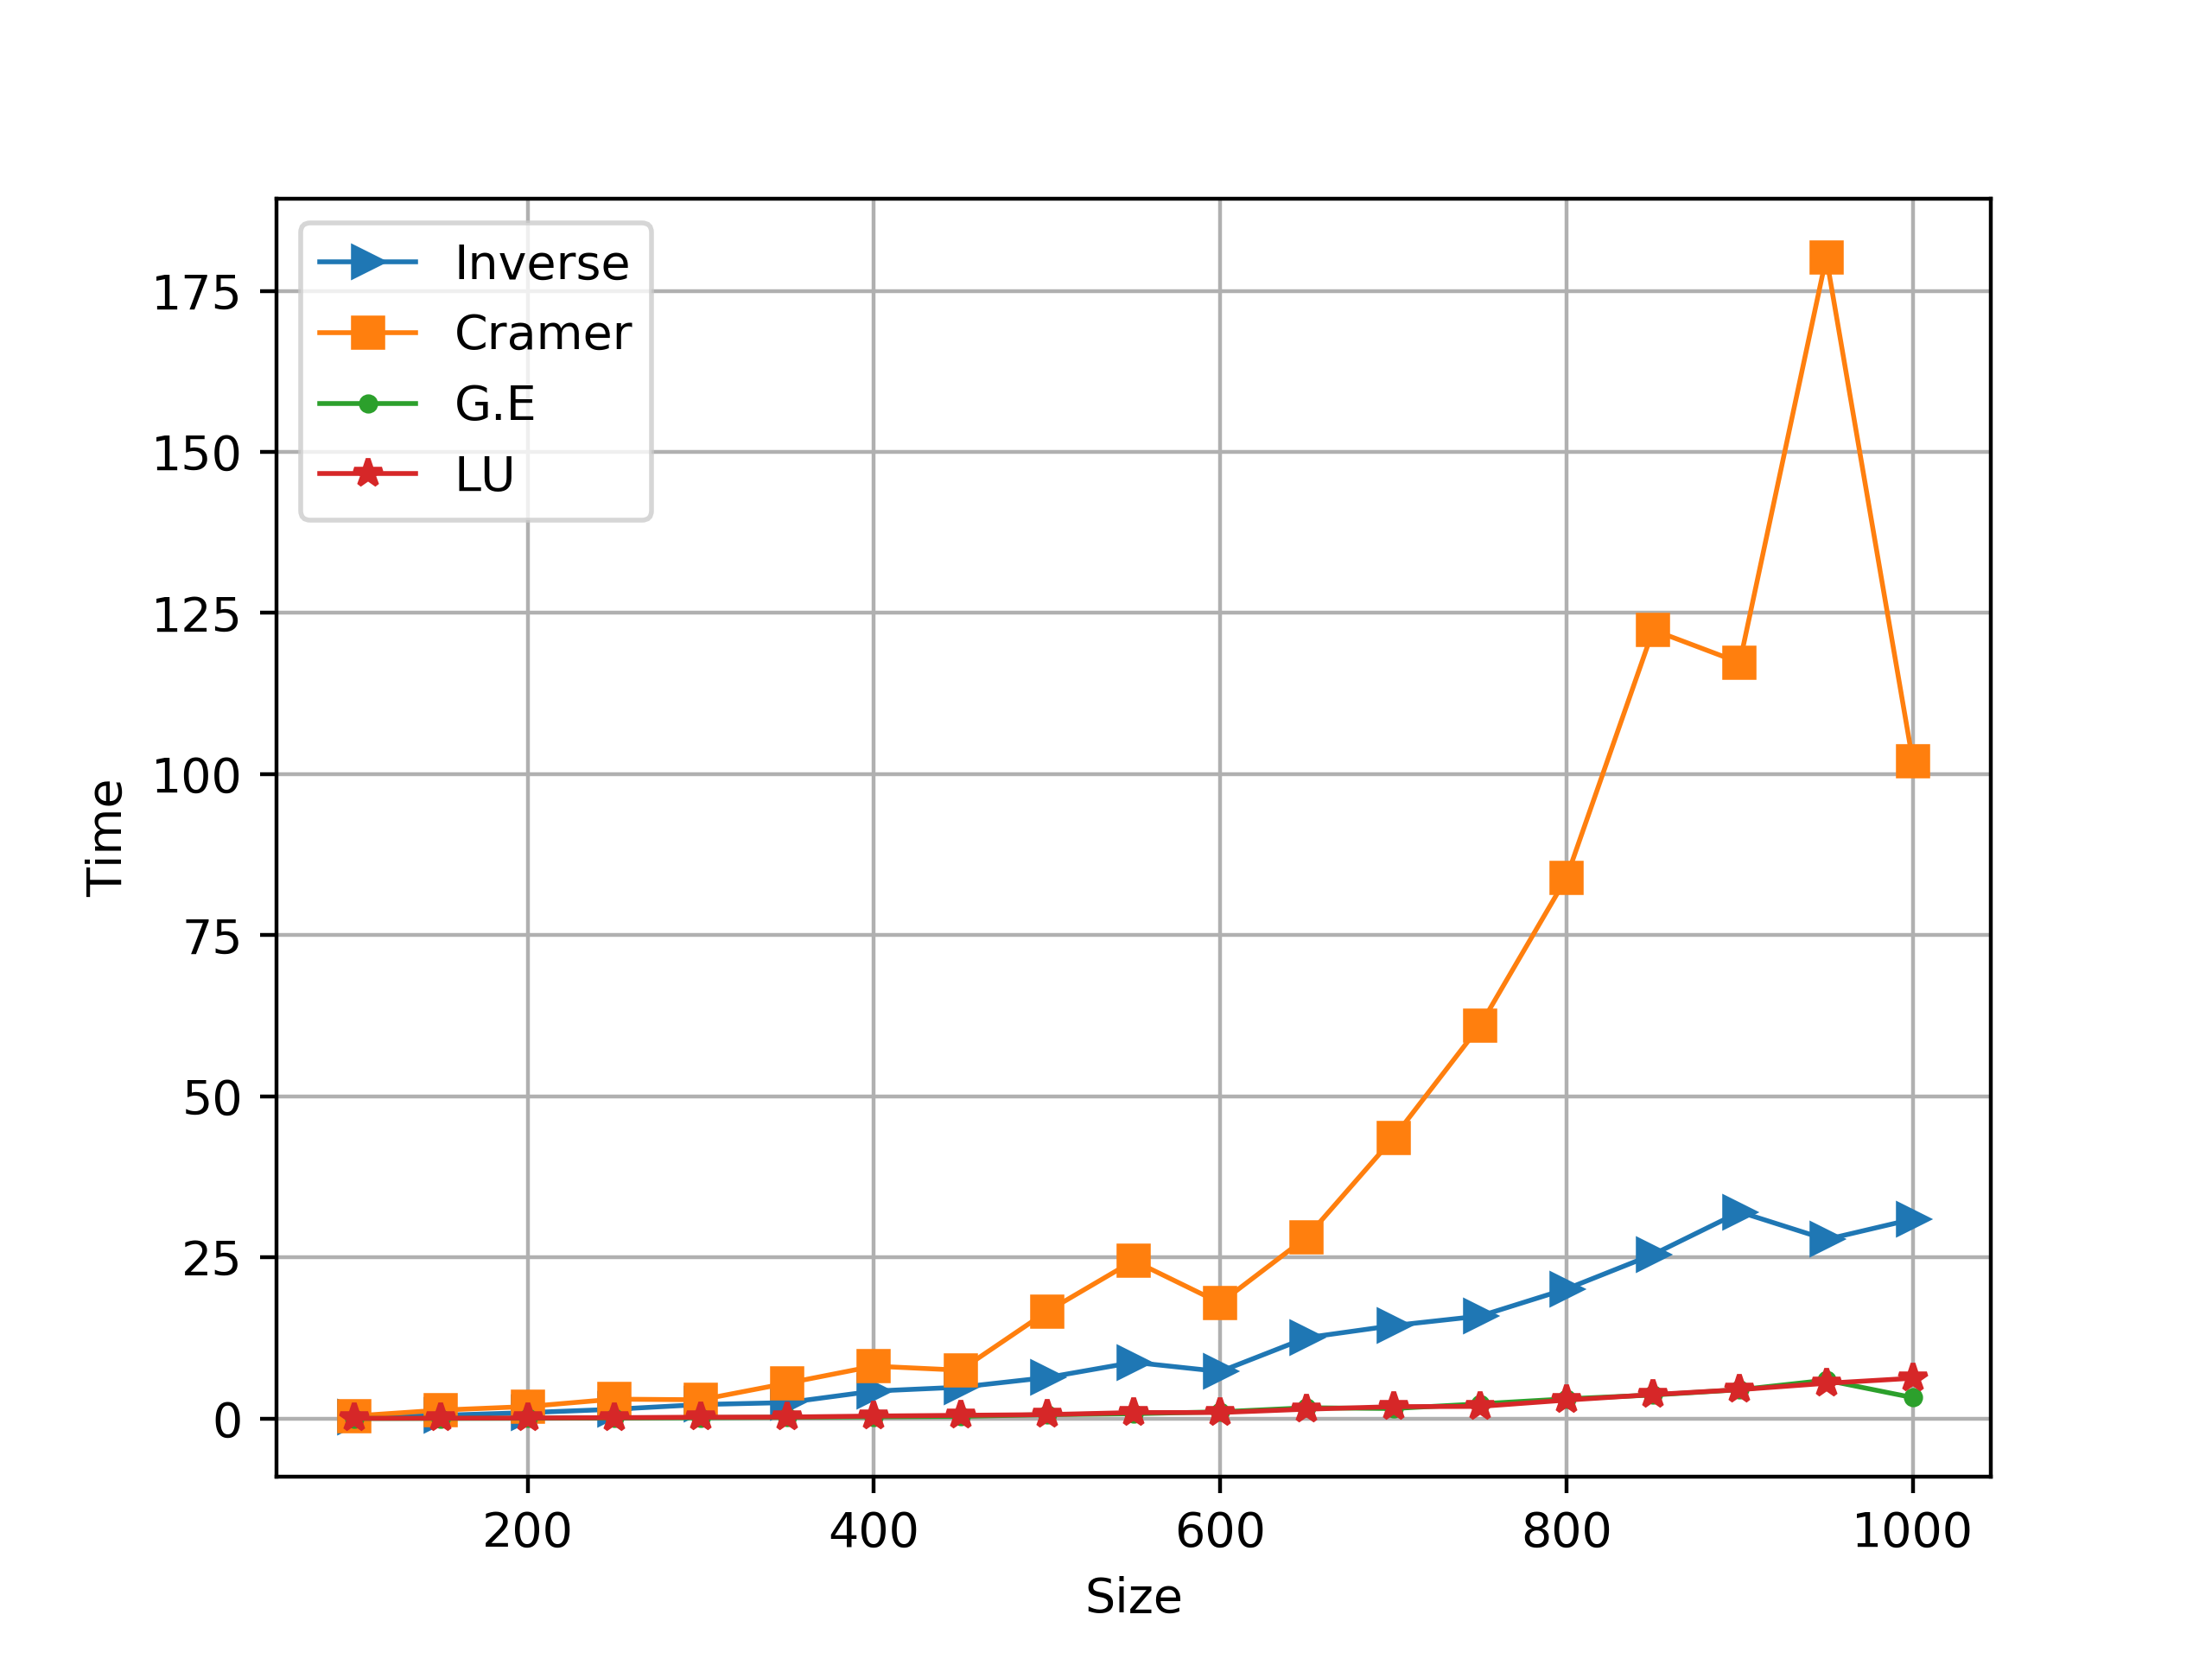
\includegraphics[width=15cm]{Plot.png}
\end{figure} 
\end{enumerate}

\newpage

\section{Roundoff Error}
\noindent\textbf{Problem 7} \textcolor{blue}{(Bonus Problem: 10 points + 8 points + 2 points)}

Given a matrix $\mathbf{A}\in \mathbb{R}^{n\times n}$, consider the roundoff error in the process of solving $\mathbf{A}\bf{x} = \bf{b}$ by Gaussian elimination in three stages:
\begin{enumerate}
    \item[1.] Decompose $\mathbf{A}$ into $\mathbf{L}\mathbf{U}$, in a machine with roundoff error $\mathbf{E}$, $\bar{\mathbf{L}}$ and $\bar{\mathbf{U}}$ are computed instead, i.e., 
    \begin{equation*}
        \mathbf{A} + \mathbf{E} = \bar{\mathbf{L}}\bar{\mathbf{U}}\,.
    \end{equation*}
    \item[2.] Solving $\mathbf{L}\bf{y} = \bf{b}$, numerically with roundoff error $\delta \mathbf{\bar{L}}$, $\hat{\mathbf{y}} = \bf{y}+\delta \bf{y}$ are computed instead, i.e.,
    \begin{equation*}
        (\bar{\mathbf{L}}+\delta \bar{\mathbf{L}})(\bf{y}+\delta \bf{y}) = \bf{b}\,.
    \end{equation*}
    \item[3.] Solving $\mathbf{U}\bf{x} = \bf{y}$, numerically with roundoff error $\delta \mathbf{\bar{U}}$, $\hat{\bf{x}} = \bf{x}+\delta \bf{x}$ are computed instead, i.e.,
    \begin{equation*}
        (\bar{\mathbf{U}}+\delta \bar{\mathbf{U}})(\bf{x}+\delta \bf{x}) = \hat{y}\,.
    \end{equation*}
\end{enumerate}
Finally, we can get the computed solution $\hat{\bf{x}}$ and 
\begin{align*}
    \bf{b} = &(\bar{\mathbf{L}}+\delta \bar{\mathbf{L}})(\bar{\mathbf{U}}+\delta \bar{\mathbf{U}})(\bf{x}+\delta \bf{x})\\
     = & (\mathbf{A}+\delta \mathbf{A})(\bf{\bf{x}}+\delta \bf{\bf{x}})\,.
\end{align*}

\begin{enumerate}
    \item Prove that the relative error of $\bf{x}$ has an upper bound as follows,
    \begin{equation*}
        \frac{\|\hat{\mathbf{x}}-\mathbf{x}\|}{\|\mathbf{x}\|} = \frac{\|\delta \bf{x}\|}{\|\bf{x}\|} \leq \frac{1}{1-\kappa(\mathbf{A})\frac{\|\delta \mathbf{A}\|}{\|\mathbf{A}\|}}\kappa(\mathbf{A})\frac{\|\delta \mathbf{A}\|}{\|\mathbf{A}\|},
    \end{equation*}
    where $\kappa(\mathbf{A}) = \|\mathbf{A}\|\|\mathbf{A}^{-1}\|$ denotes the condition number of matrix $\mathbf{A}$ (Suppose $\mathbf{A}$ and $\mathbf{A}+\delta \mathbf{A}$ are nonsingular and $\|\mathbf{A}^{-1}\|\|\delta \mathbf{A}\|<1$), and $\|\cdot\|$ can be any norm.
    
    \textbf{Hint}: The following equation might be useful,
    \begin{align*}
        \|(\mathbf{I}-\mathbf{B})^{-1}\| =  \|\sum_{k = 0}^{\infty} \mathbf{B}^k\| \leq \sum_{k = 0}^{\infty} \|\mathbf{B}\|^k \leq  \frac{1}{1-\|\mathbf{B}\|}\,.
    \end{align*}
    
    % \begin{equation}
    %     (\mathbf{I}-\mathbf{A})^{-1} = \mathbf{I} + \mathbf{A} + \mathbf{A}^2 + ... = \sum_{k = 0}^\infty \mathbf{A}^{k},
    % \end{equation}
    
    where $\mathbf{I}-\mathbf{B}$ is nonsingular and $\lim_{n\to \infty}\mathbf{B}^n = \mathbf{0}$.
    
    \item Consider a linear system $\mathbf{A}\mathbf{x} = \mathbf{b}$, where
    
    \[
        \mathbf{A} = \begin{bmatrix}2 & -1 & 1 \\ -1 &10^{-10} &10^{-10}\\ 1 & 10^{-10} & 10^{-10}  \end{bmatrix},\quad \mathbf{b} = \begin{bmatrix}2(1+10^{-10}) \\ -10^{-10} \\10^{-10} \end{bmatrix}
    \]
    
    find the solution $\mathbf{x}$, and calculate the condition number of $\mathbf{A}$ with the matrix infinite norm\footnote{If $\mathbf{A}\in\mathbb{R}^{n\times n}$, then the matrix infinite norm is  $\|\mathbf{A}\|_{\infty} = \max_{1<i<n}\sum_{j = 1}^n|a_{i,j}|$.}, i.e. $\kappa_\infty(\mathbf{A}) = \|\mathbf{A}\|_\infty\|\mathbf{A}^{-1}\|_\infty$. Suppose $|\delta\mathbf{A}|<10^{-18}|\mathbf{A}|$\footnote{$|\mathbf{A}|\leq |\mathbf{B}|$ means each element in $\mathbf{A}$ is relative smaller to the corresponding element of $\mathbf{A}$}, use $\kappa_\infty(\mathbf{A})$ to verify that 
    \[
        \|\delta \mathbf{x}\|< 10^{-7} \|\mathbf{x}\|. 
    \]
    
    
    \item Discuss what you have observed from the previous 2 questions. What are the main factors that influence the relative error of the computed solution? Does the ill-conditioned matrix (i.e. the condition number is large) always lead to a large error of the solution?     
\end{enumerate}

\noindent\textbf{Solution.}
\begin{enumerate}
    \item 
    This original question is equivalent to prove
    \begin{align*}
    \frac{||\delta x||}{||x||} &\le \frac{||A^{-1}||||\delta A|| -1 + 1}{1-||A^{-1}||||\delta A||}\\
    &\le \frac{1}{1-||A^{-1}||||\delta A||}-1\\
   \rightarrow \frac{||\delta x|| + ||x||}{||x||} &\le \frac{1}{1-||A^{-1}\delta A||}\\
    \rightarrow||\delta x|| &\le ||A^{-1}\delta A||(||\delta x|| + ||x||)\\
    \end{align*}
    By the property of norm, we need to prove
    \begin{align*}
    ||\delta x||&\le ||A^{-1}\delta A \delta x|| + ||A^{-1}\delta A x||\\
    \rightarrow ||\delta x|| &\le ||A^{-1}\delta A(x+\delta x)|| \\
    \le 
    \end{align*}
    Since 
    $$(A+\delta A)(x+\delta x) = Ax \Leftrightarrow \delta Ax + \delta A \delta x + A\delta x = 0$$
    we have
    $$||\delta x|| = ||A^{-1}(-\delta Ax - A\delta x)||=||A^{-1}\delta A x + \delta x||\ge ||A^{-1}\delta A x + A^{-1}\delta A x||$$
   	So we need to prove
   	$$||\delta x|| \le ||A^{-1}\delta A(x+\delta x)||\le ||\delta x||$$
   	This is obviously true. Q.E.D
    \item 
    \item
    
\end{enumerate}

\end{document}
